%% SECTION HEADER /////////////////////////////////////////////////////////////////////////////////////
\section{The \acl{madif} determination at various ambient temperatures}
\label{sec:madifTemp}

%% SECTION CONTENT ////////////////////////////////////////////////////////////////////////////////////
In addition to the referenced \ac{madif} obtained for +20\unit{\degreeCelsius}, a study of wave propagation at temperatures T=\(\left[-10,\,0,\,+10,\,+30,\,+40,\,+50\right]\)\unit{\degreeCelsius} was carried out.
To determine temperature-dependent \ac{gw} propagation in \ac{hsc} using simulations, the material properties of the components were assumed according to the methodology described in Section~\ref{sec:temp}.

The temperature effect on the \acp{madif} was developed based on the \ac{fcgm} and removed interface elements as a damage model.
The analysis used both \acp{di}, i.e. the \ac{rmsd} and the \ac{cc}, for the 100 \unit{\kHz} full-length signals.
The signals obtained for a healthy sample at considered temperatures were taken as the reference signals for each case.
As with the reference temperature, an analysis of the selection of the fitting function was performed.
The best results were obtained for Eq.~(\ref{eq:function_1}), and the function coefficients for each temperature are collected in Table~\ref{tab:fit_F_err_temp}.
\begin{table}[!tbh]
	\small
	\tabcolsep=0.25cm
	\centering
	\caption{\label{tab:fit_F_err_temp} The coefficients of the function from Eq.~(\ref{eq:function_1}) fitted to the \aclp{madif} based on the \acl{fcgm} - interface at 100 \unit{\kHz} for various ambient temperatures}
	\begin{tabular}{cccccccc}
		\toprule
		{T \unit{\degreeCelsius}} & Eq.~(\ref{eq:function_1}) & -10 & 0 & +10 & +30 & +40 & +50\\
		\midrule
		\multirow{3}{*}{\ac{rmsd}} & $a_1$ & 11.116 & 10.881 & 13.198 & 11.371 & 9.487 & 9.798\\
		 & $a_2$ & 29.874 & 31.651 & 36.911 & 34.972 & 32.009 & 34.369\\
		 & $a_3$ & 0.661 & 0.656 & 0.642 & 0.675 & 0.704 & 0.715\\
		\midrule
		\multirow{3}{*}{\ac{cc}} & $a_1$ & 28.002 & 19.543 & 24.902 & 8.472 & 4.831 & 4.104\\
		& $a_2$ & 182.741 & 145.820 & 167.862 & 92.602 & 70.548 & 70.889\\
		& $a_3$ & 0.847 & 0.866 & 0.852 & 0.909 & 0.932 & 0.942\\
		\bottomrule
	\end{tabular}
\end{table}

The temperature-dependent \acp{madif} based on the \ac{rmsd} and the \ac{cc} are presented in Figures~\ref{fig:madif_temp_rmsd} and \ref{fig:madif_temp_cc}, respectively.
It is observed that the variation in ambient temperature condition can substantially influence the \ac{madif} values.
The numerical results were in good agreement with the experimental measurements for the ambient temperature over 0\unit{\degreeCelsius} (Figure~\ref{fig:madif_temp_rmsd}).
The results obtained at 0\unit{\degreeCelsius} and -10\unit{\degreeCelsius} have a much larger error because the model-based functions tend to have a lower value than the experimental ones.
Therefore, the assumed linear model of the temperature-dependent material properties of the components used in the simulation was not sufficiently accurate with the real object.
\begin{figure}[!tbh]
	\begin{center}
		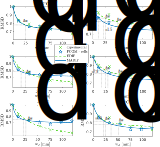
\includegraphics[width=0.95\textwidth]{Chapter_8/MADIF_temp_RMSD}
	\end{center}
	\caption{The \acf{madif} and the \acf{edif} based on the \acf{rmsd} 100 \unit{\kHz}}
	\label{fig:madif_temp_rmsd}
\end{figure}
\begin{figure}
	\begin{center}
		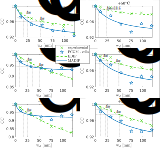
\includegraphics[width=0.95\textwidth]{Chapter_8/MADIF_temp_CC}
	\end{center}
	\caption{The \acf{madif} and the \acf{edif} based on the \acf{cc} 100 \unit{\kHz}}
	\label{fig:madif_temp_cc}
\end{figure}
In the case of the \ac{cc}, the best results were achieved at temperatures between +10\unit{\degreeCelsius} and +40\unit{\degreeCelsius}.
\clearpage